% Kyla Andersen USP proposal
\documentclass[12pt]{article}
\usepackage[margin=1in]{geometry}
\usepackage{setspace}
\usepackage{amsmath, amssymb}
\usepackage{graphicx}
\usepackage{hyperref}
\usepackage{natbib}
\usepackage{wrapfig}
\bibliographystyle{plain}

% Begin document
\begin{document}

% Title Section
\title{Topological Trait Estimation for Phylogenetic Reconstruction of Fossil
Evolution}
\author{Kyla Andersen}
\date{08/30/2024}
\maketitle

% Double spacing
\doublespacing

% Section 1: Introduction
\section{Introduction}
\begin{wrapfigure}{R}{0.3\textwidth}
	\centering
	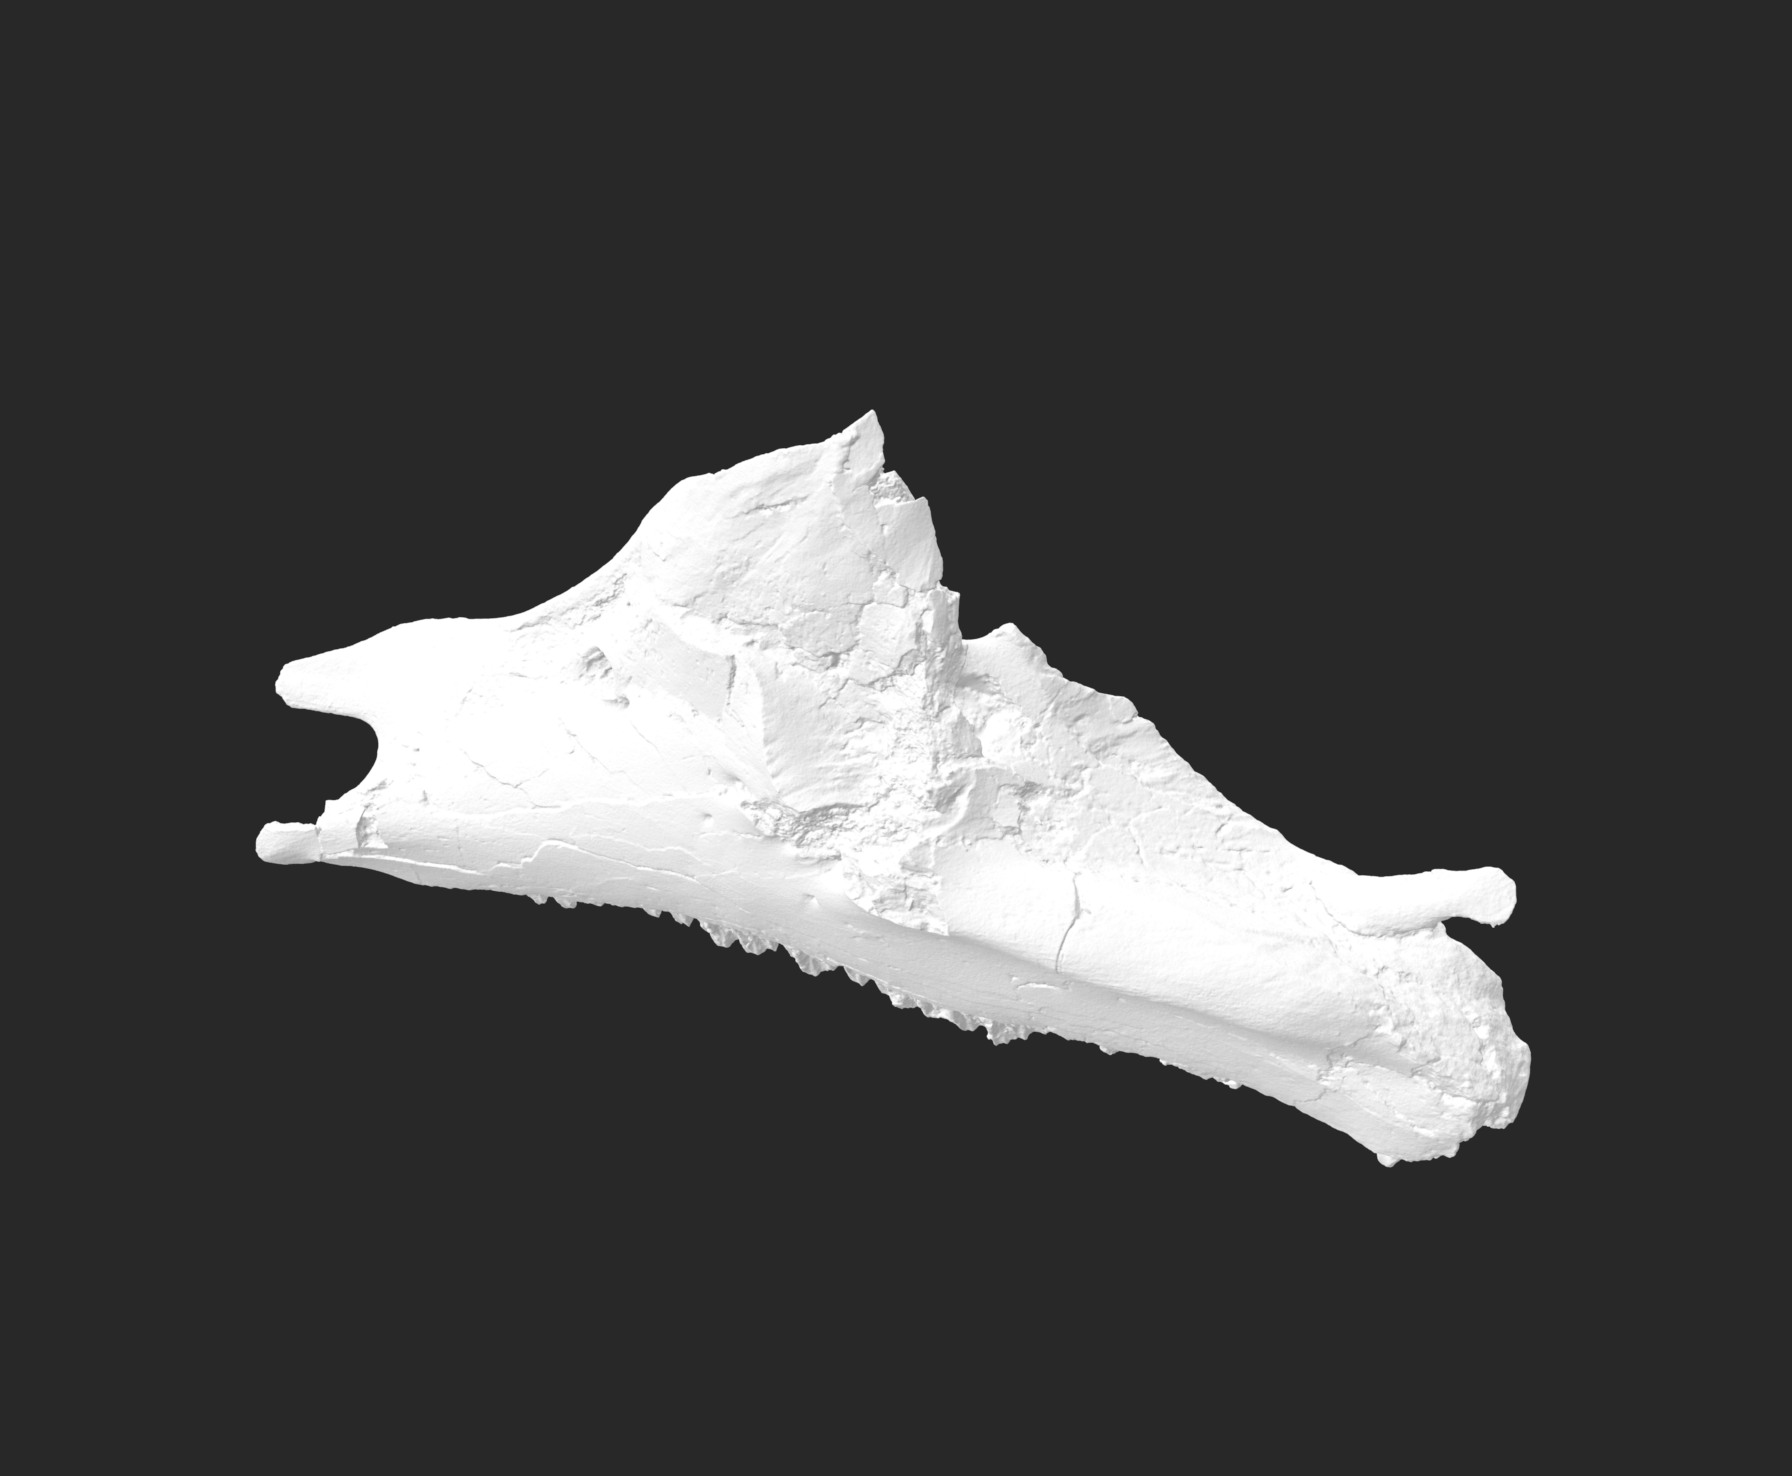
\includegraphics[width=0.4\textwidth]{dino_bone.png}
	\caption{A  3D scan of the left maxilla of an Edmontosaurus.}
	\label{fig:dino_maxilla}
\end{wrapfigure}

Topological methods have emerged as powerful tools in data analysis,
particularly for complex, high-dimensional datasets such as those found in
paleontology. The study of dinosaur evolution, traditionally reliant on
morphological analysis of fossilized bones, is an area ripe for innovation
through these topological techniques. \autoref{fig:dino_maxilla} shows how a dinosaur fossil can
be scanned and turned into a 3D image. Estimating morphological traits from 3D
scans of bones can provide insights into the evolutionary relationships between
different species and offer a clearer picture of their lineage and adaptations
over time. 

Current approaches to this problem involve manually entering and comparing the 
morphological data, a process that is not only time-consuming but also prone to
human error and subjectivity \citep{bates2009}. One computational approach, topological 
data analysis (TDA), offers a mathematical framework that captures the intrinsic 
geometric and topological properties of shapes, allowing for a more robust and 
efficient method of trait estimation. Unlike traditional methods, TDA can handle 
variations in shape, scale, and orientation, which enables more accurate
comparisons of complex structures \citep{zomorodian2009}.

In analyzing the traits of dinosaur bones, TDA would allow researchers to quantify
differences and similarities by representing the shapes as high-dimensional data
points. By treating these shapes as topological spaces, it becomes possible to
construct a phylogenetic tree that reflects the true evolutionary history of a
given species with greater precision and less manual intervention \citep{yang2012}.
A phylogenetic tree is a diagram that displays the lines of evolutionary descent
of different species. By using the traits found on certain dinosaur fossils, I
will draw my own tree with good resolution by identifying key morphological 
features that suggest specific evolutionary branches or relationships. This is 
the area I wish to further study, particularly for its potential to enhance our 
understanding of evolutionary relationships. 

% Section 2: Background
\section{Background}
\begin{wrapfigure}{R}{0.3\textwidth}
	\centering
	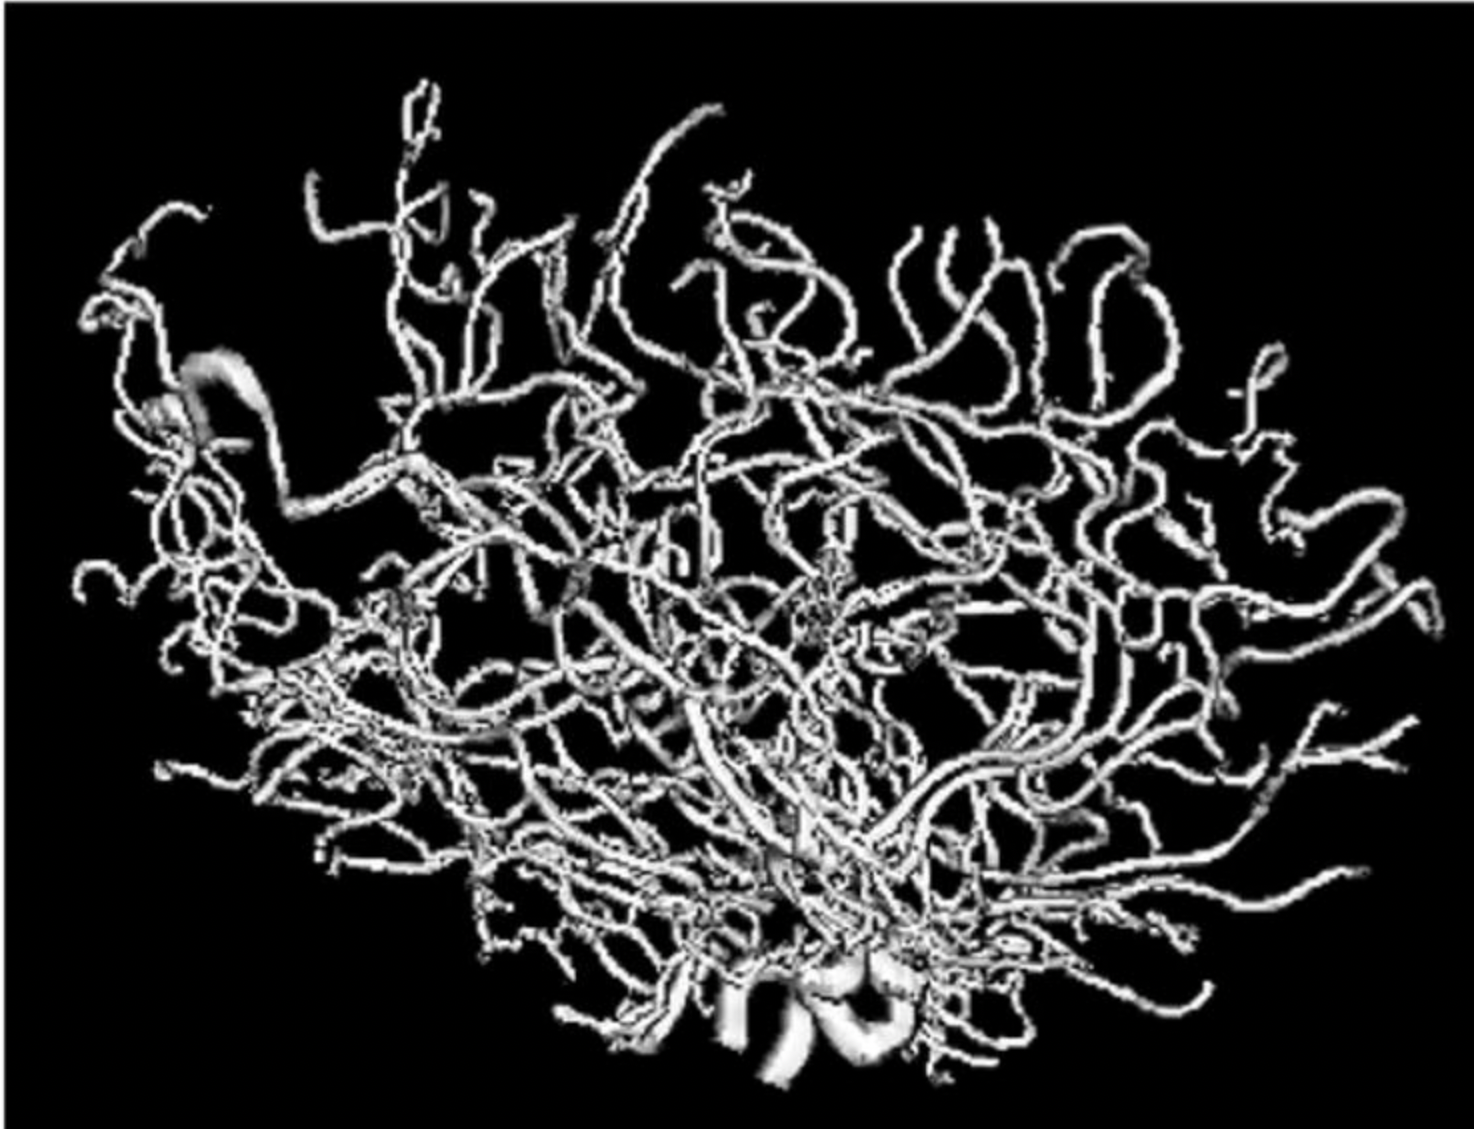
\includegraphics[width=0.3\textwidth]{arteryTree.png}
	\caption{By using tools from TDA, \cite{bendich2016} uncovered previously
unknown traits of the complex branching structure of arteries, as seen here}
	\label{fig:artery_tree}
\end{wrapfigure}
Recent studies have demonstrated the power of TDA in fields such as neuroscience
and anatomy. Notably, Bendich et al. \cite{bendich2016} utilized 
TDA to analyze brain artery structures, revealing correlations between age, sex, 
and the bending of arteries that were not present in previous studies. In
\autoref{fig:artery_tree}, we see how an artery is constructed and then studied 
using various techniques. TDA methods provide new insights into complex 
data by capturing changes in the connectedness of structures and enabling the 
analysis of high-dimensional characteristics, such as shape and form, often 
overlooked by traditional metrics. 

%\begin{wrapfigure}{R}{0.3\textwidth}
%	\centering
%	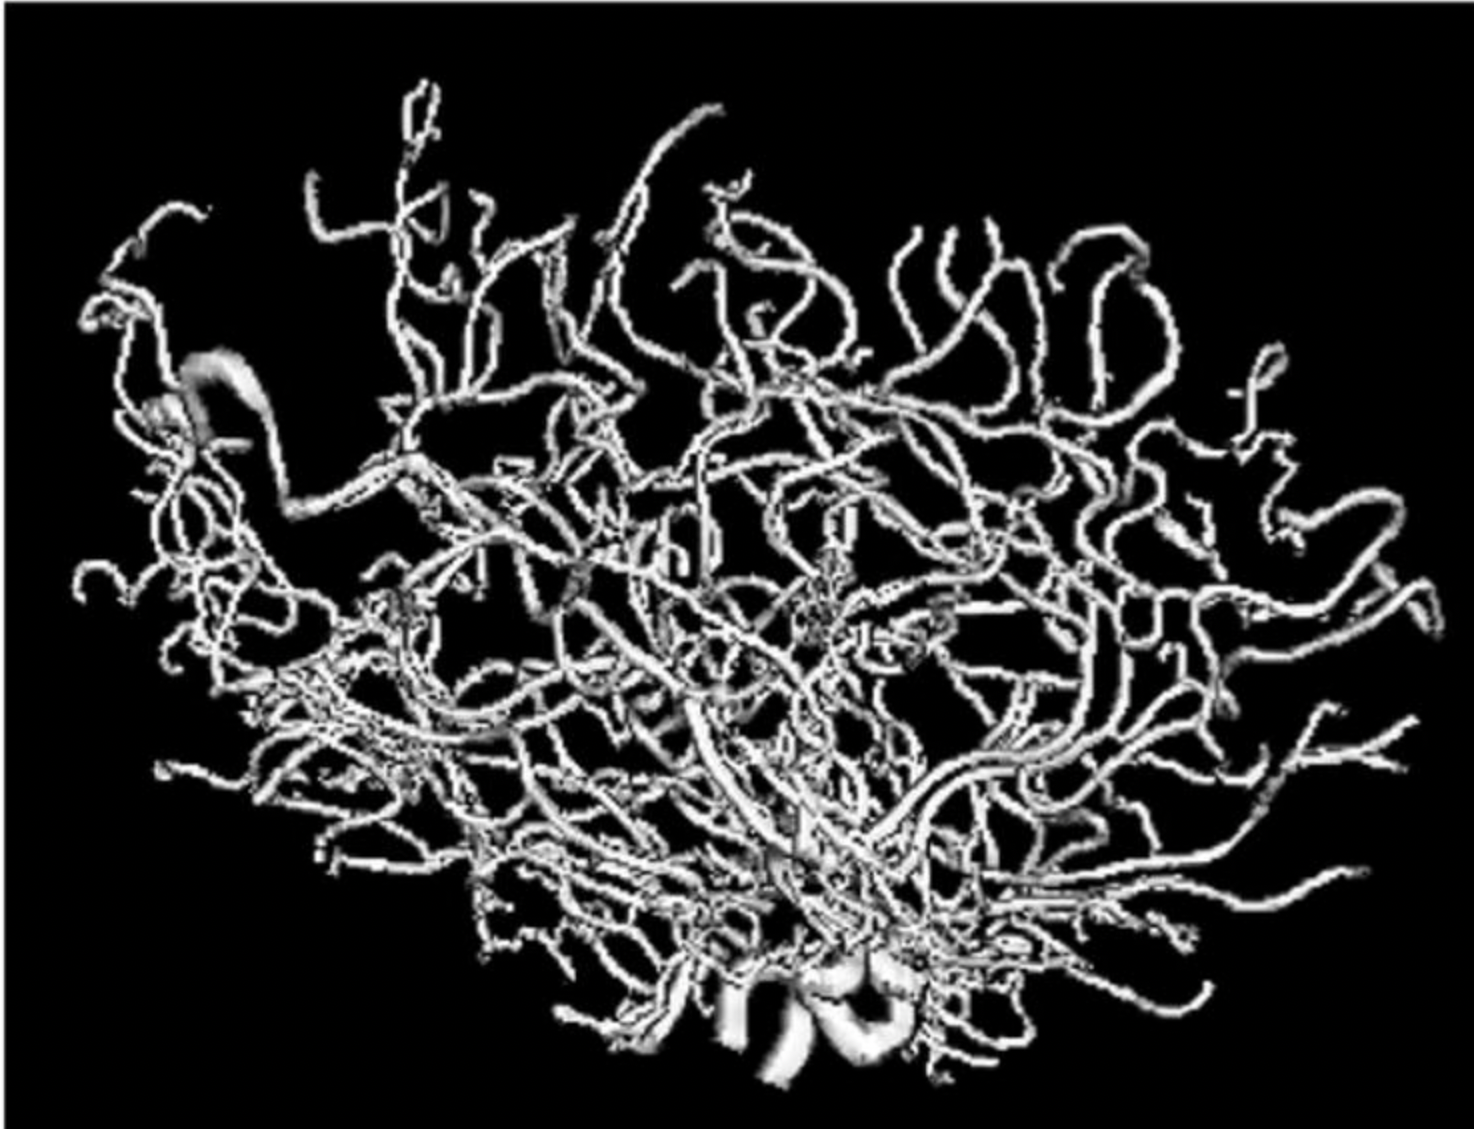
\includegraphics[width=0.3\textwidth]{arteryTree.png}
%	\caption{By using tools from TDA, \cite{bendich2016} uncovered previously
%unknown traits of the complex branching structure of arteries, as seen here}
%	\label{fig:artery_tree}
%\end{wrapfigure}

With advancements in 3D imaging and data acquisition technologies, applying TDA 
to 3D data feature simplification has gained significant
traction in recent years. A study produced by Ou Li \citep{li2021} introduced a 
method that leverages TDA for segmenting and simplifying 3D point cloud data, a
representation commonly only obtained through low-cost 3D sensors. 
The study demonstrated that TDA can effectively partition complex, disorganized 
3D data into subsets with consistent characteristics, using various techniques 
that simplify the data structure while retaining critical geometric information
\citep{li2021}.

Dornbusch et al. \cite{dornbusch2007}, developed a method that utilizes 3D point 
clouds to extract and parameterize morphological traits of plant organs, which 
are then used to create a comprehensive architectural model of the plant. Fitting 
these 3D point clouds into a structural model, the method enables a precise 
portrayal of the leaf and stem shape and their spatial orientations \citep{dornbusch2007}. 
By applying this technique to 3D scans of fossils, one can extract and parameterize 
various morphological traits, such as bone structure and dimensions, with high 
accuracy. This detailed characterization allows for reconstructing more exact
evolutionary trees and a better understanding of the anatomical variations among
different species. Integrating this approach will significantly enhance the
ability to trace evolutionary relationships and track the development of
specific traits over time. 

While computational methods for analyzing 3D scans have advanced significantly
in fields like medical imaging and industrial design, paleontology has not yet
fully leveraged these tools. Current research in paleontology has a noticeable lack of
specialized algorithms and methods tailored for interpreting the complex,
irregular shapes of fossilized remains, such as dinosaur bones. The gap lies in
the adaptation and development of these advanced computational methods to suit
the specific challenges of paleontological data.

Building on existing research in 3D scan analysis and computational methods, my
goal is to advance these techniques more specifically for the field of
paleontology. By applying and adapting algorithms such as the one used by
Dornbusch et al. \citep{dornbusch2007}, I aim to develop new methods for analyzing 
and characterizing dinosaur bones from 3D scans. This work seeks to fill the 
current gap in applying these advanced techniques to paleontological data, 
ultimately improving the accuracy of evolutionary trees and our understanding of 
prehistoric life. I will ensure the accuracy of my phylogenetic tree through
comparissons of known fossil relatives that have been hand caluclated and use
those results to validate the methods I choose.

I look forward to expanding my research experience by taking on the challenge of
an independent project for the first time. With a solid background in
coding with Python, Java, and C++, I have the skills that will be instrumental 
in developing and implementing the new algorithms necessary for this research. 
This project will allow me to deepen my knowledge of computational topology and 
enhance my skills in algorithm development and data analysis. I am eager to 
contribute to the field of paleontology with a tool that not only advances our 
capability to analyze fossil data but also has the potential to influence broader 
applications in scientific research.

% Section 3: Methods
\section{Methods}
To begin this project, I will preprocess 3D scans of dinosaur bones to clean and
normalize the data. Specifically, I will ensure consistency in scale, orientation, and resolution
by removing noise, filling holes, and aligning scans using tools from Python,
such as trimesh and pygltflib. Next, I will adapt existing algorithms, such as
point cloud registration and surface fitting to identify key morphological
features of the bones. This will involve implementing and customizing these
algorithms in Python, utilizing libraries like NumPy, SciPy, and PyTorch.
Following this, I will develop new algorithms specifically tailored to
paleontology, using techniques like principal component analysis (PCA) and
singular value decomposition (SVD) to analyze and compare features across specimens.
Certain machine learning models, such as convolutional neural networks (CNN) may also
be utilized to enhance automated characterization. Experiments will validate the
effectiveness of these methods by comparing them to known data, using metrics
like shape similarity scores and classification accuracy to ensure robustness
across different types of bones. The final stage will involve documenting the
findings in an abstract or research paper, which will highlight the
potential applications of these methods in paleontology and beyond.

% Section 4: Timeline
\section{Timeline}
An outline of the estimated timeline for this project is listed below.

\begin{enumerate}
	\item Clean, normalize, and align 3D scans using \texttt{trimesh} and
	\texttt{pygltflib}: 2 weeks
	\item Implement and adapt existing algorithms to identify key morphological
	features of the bones: 3 weeks
	\item Develop and customize new algorithms tailored to paleontology using
	PCA, SVD and CNNs to enhance automated characterization: 5 weeks
	\item Conduct experiments to validate methods, comparing them to known data:
	3 weeks
	\item Analyze the results, refine methods as needed, and compile findings
	for documentation: 3 weeks
%	\item Assemble my finding for an abstract or research paper: 1 week
\end{enumerate}

% Section 5: Collaboration with Faculty Sponsor
\section{Collaboration with Faculty Sponsor}
My primary faculty sponsor for this project is Dr. Brittany Fasy, whose ongoing
research in 3D shape analysis aligns with the methodological aspects of this
project. I plan to meet with Dr. Fasy regularly as her expertise in computational 
geometry and 3D data analysis will be invaluable in guiding the development and 
refinement of algorithms for this project. Additionally, I will be collaborating 
with Dr. Christopher Organ, whose work in evolutionary biology and paleontology 
will provide crucial insights into the biological relevance of the morphological 
features I am going to analyze. I am eager to engage in this research project, 
which not only supports the work of my mentors but also aims to make a meaningful 
contribution to the fields of computational topology and paleontology.

\newpage

% Section 6: References
\bibliography{ref.bib} 

\end{document}


